\section{eo\-Quad2Bin\-Op$<$ EOT $>$ Class Template Reference}
\label{classeo_quad2_bin_op}\index{eoQuad2BinOp@{eoQuad2BinOp}}
Turning an {\bf eo\-Quad\-Op}{\rm (p.\,\pageref{classeo_quad_op})} into an {\bf eo\-Bin\-Op}{\rm (p.\,\pageref{classeo_bin_op})}: simply don't touch the second arg!  


{\tt \#include $<$eo\-Op.h$>$}

Inheritance diagram for eo\-Quad2Bin\-Op$<$ EOT $>$::\begin{figure}[H]
\begin{center}
\leavevmode
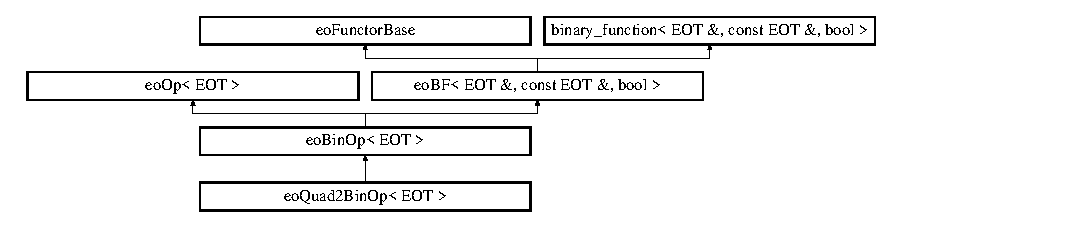
\includegraphics[height=2.60163cm]{classeo_quad2_bin_op}
\end{center}
\end{figure}
\subsection*{Public Member Functions}
\begin{CompactItemize}
\item 
{\bf eo\-Quad2Bin\-Op} ({\bf eo\-Quad\-Op}$<$ {\bf EOT} $>$ \&\_\-quad\-Op)
\begin{CompactList}\small\item\em Ctor. \item\end{CompactList}\item 
bool {\bf operator()} ({\bf EOT} \&\_\-eo1, const {\bf EOT} \&\_\-eo2)\label{classeo_quad2_bin_op_a1}

\begin{CompactList}\small\item\em Operator() simply calls embedded quad\-Op operator() with dummy second arg. \item\end{CompactList}\end{CompactItemize}
\subsection*{Private Attributes}
\begin{CompactItemize}
\item 
{\bf eo\-Quad\-Op}$<$ {\bf EOT} $>$ \& {\bf quad\-Op}\label{classeo_quad2_bin_op_r0}

\end{CompactItemize}


\subsection{Detailed Description}
\subsubsection*{template$<$class EOT$>$ class eo\-Quad2Bin\-Op$<$ EOT $>$}

Turning an {\bf eo\-Quad\-Op}{\rm (p.\,\pageref{classeo_quad_op})} into an {\bf eo\-Bin\-Op}{\rm (p.\,\pageref{classeo_bin_op})}: simply don't touch the second arg! 



Definition at line 143 of file eo\-Op.h.

\subsection{Constructor \& Destructor Documentation}
\index{eoQuad2BinOp@{eo\-Quad2Bin\-Op}!eoQuad2BinOp@{eoQuad2BinOp}}
\index{eoQuad2BinOp@{eoQuad2BinOp}!eoQuad2BinOp@{eo\-Quad2Bin\-Op}}
\subsubsection{\setlength{\rightskip}{0pt plus 5cm}template$<$class EOT$>$ {\bf eo\-Quad2Bin\-Op}$<$ {\bf EOT} $>$::{\bf eo\-Quad2Bin\-Op} ({\bf eo\-Quad\-Op}$<$ {\bf EOT} $>$ \& {\em \_\-quad\-Op})\hspace{0.3cm}{\tt  [inline]}}\label{classeo_quad2_bin_op_a0}


Ctor. 

\begin{Desc}
\item[Parameters:]
\begin{description}
\item[{\em \_\-quad\-Op}]the {\bf eo\-Quad\-Op}{\rm (p.\,\pageref{classeo_quad_op})} to be transformed \end{description}
\end{Desc}


Definition at line 149 of file eo\-Op.h.

The documentation for this class was generated from the following file:\begin{CompactItemize}
\item 
eo\-Op.h\end{CompactItemize}
